\documentclass[border=0.5mm]{standalone}

\usepackage{import}
\subimport{../../../}{preamble.tex}

\usepackage{tikz}
\usetikzlibrary{calc}

\usepackage{pgfplots}
\usepgfplotslibrary{fillbetween}

\begin{document}

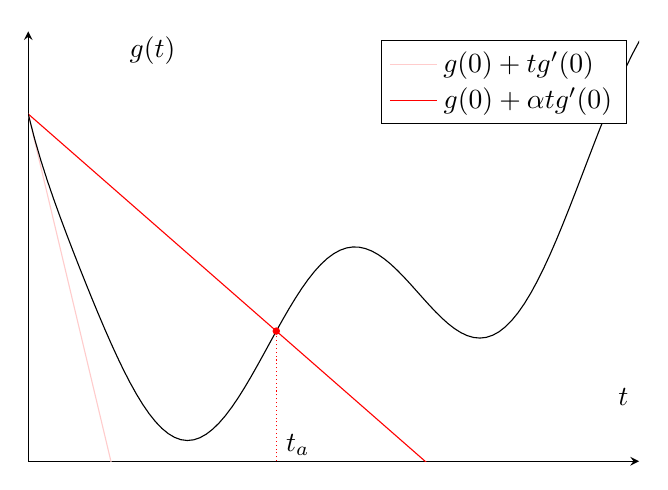
\begin{tikzpicture}

  \begin{axis}[
    ticks=none,
    axis lines=left,
    y=0.7cm,            % y unit vector
    x=4cm,            % x unit vector
    clip=true,
    xmin=0,
    ymin=3.2,
    ymax=11,
    xlabel={$t$},
    ylabel={$g(t)$},
    x label style={at={(axis description cs:0.95,0.15)},anchor=west},
    y label style={at={(axis description cs:0.15,0.9)},rotate=-90,anchor=south west},
    clip=true
    ]

    \addplot[mark=none, red!20, samples=100, domain=0:2] { 9.5-24*x};
    \addlegendentry{$g(0)+t g'(0)~~$}
    \addplot[mark=none, red, samples=100, domain=0:2] { 9.5-5*x};
    \addlegendentry{$g(0)+\alpha t g'(0)$}
    
    \addplot[mark=none, black, samples=100, domain=0:2] {2 +1/(0.2+x) + 1.5*cos(360*x) + exp(x) };

    \node[circle, draw=red, fill=red, inner sep=0.8] at (axis cs: 0.7876, 5.56175) {};
    \draw[draw=red, densely dotted] (axis cs: 0.7876, 3.2) -- (axis cs: 0.7876, 5.56175);
    \node[right] at (axis cs: 0.7876, 3.5) {$t_a$};

    
    
  \end{axis}  
\end{tikzpicture}

\end{document}

%%% Local Variables:
%%% mode: latex
%%% TeX-master: t
%%% End:
